    %% Le lingue utilizzate, che verranno passate come opzioni al pacchetto babel. Come sempre, l'ultima indicata sar� quella primaria.
%% Se si utilizzano una o pi� lingue diverse da "italian" o "english", leggere le istruzioni in fondo.
\def\thudbabelopt{english,italian}


%% Valori ammessi per target: bach (tesi triennale), mst (tesi magistrale), phd (tesi di dottorato).
%% Valori ammessi per aauheader: '' (vuoto -> nessun header Alpen Adria Univeristat), aics (Department of Artificial Intelligence and Cybersecurity), informatics (Department of Informatics Systems). Il nome del dipartimento � allineato con la versione inglese del logo UniUD.
%% Valori ammessi per style: '' (vuoto -> stile moderno), old (stile tradizionale).
\documentclass[target=bach,aauheader=,style=]{thud}
\usepackage{graphicx}
\usepackage{wrapfig}
\usepackage{placeins}
\graphicspath{ {./images/} }
%% --- Informazioni sulla tesi ---
%% Per tutti i tipi di tesi
% Scommentare quello di interesse, o mettete quello che vi pare

\course{Internet of Things, Big Data e Machine Learning}

\title{titolo \\ work in \\ progress }
\author{Campo Lorenzo}
\supervisor{Prof.\ Vincenzo Riccio}
%\cosupervisor{Arch.\ Rambaldo Melandri \and Dott.\ Giorgio Perozzi}
\tutor{Giuliana Milan}
%% Campi obbligatori: \title, \author e \course.
%% Altri campi disponibili: \reviewer, \tutor, \chair, \date (anno accademico, calcolato in automatico), \rights
%% Con \supervisor, \cosupervisor, \reviewer e \tutor si possono indicare pi� nomi separati da \and.
%% Per le sole tesi di dottorato:
\phdnumber{313}
\cycle{XXVIII}
\contacts{Via della Sintassi Astratta, 0/1\\65536 Gigatera --- Italia\\+39 0123 456789\\\texttt{http://www.example.com}\\\texttt{inbox@example.com}}

%% --- Pacchetti consigliati ---
%% pdfx: per generare il PDF/A per l'archiviazione. Necessario solo per la versione finale
\usepackage[a-1b]{pdfx}
%% hyperref: Regola le impostazioni della creazione del PDF... pi� tante altre cose. Ricordarsi di usare l'opzione pdfa.
\usepackage[pdfa]{hyperref}
%% tocbibind: Inserisce nell'indice anche la lista delle figure, la bibliografia, ecc.

%% --- Stili di pagina disponibili (comando \pagestyle) ---
%% sfbig (predefinito): Apertura delle parti e dei capitoli col numero grande; titoli delle parti e dei capitoli e intestazioni di pagina in sans serif.
%% big: Come "sfbig", solo serif.
%% plain: Apertura delle parti e dei capitoli tradizionali di LaTeX; intestazioni di pagina come "big".

\begin{document}
\maketitle

%% Dedica (opzionale)
\begin{dedication}
	dedica%Al mio cane,\par per avermi ascoltato mentre ripassavo le lezioni.
\end{dedication}

%% Ringraziamenti (opzionali)
\acknowledgements
Sed vel lorem a arcu faucibus aliquet eu semper tortor. Aliquam dolor lacus, semper vitae ligula sed, blandit iaculis leo. Nam pharetra lobortis leo nec auctor. Pellentesque habitant morbi tristique senectus et netus et malesuada fames ac turpis egestas. Fusce ac risus pulvinar, congue eros non, interdum metus. Mauris tincidunt neque et aliquam imperdiet. Aenean ac tellus id nibh pellentesque pulvinar ut eu lacus. Proin tempor facilisis tortor, et hendrerit purus commodo laoreet. Quisque sed augue id ligula consectetur adipiscing. Vestibulum libero metus, lacinia ac vestibulum eu, varius non arcu. Nam et gravida velit.

%% Sommario (opzionale)
\abstract
Nunc ac dignissim ipsum, quis pulvinar elit. Mauris congue nec leo ornare lobortis. Nulla hendrerit pretium diam nec lobortis. Nullam aliquam laoreet nisl, sit amet facilisis lectus accumsan ut. Duis et elit hendrerit metus venenatis condimentum. Integer id eros molestie, interdum leo sit amet, aliquet metus. Integer fermentum tristique magna, vel luctus neque rhoncus vel. Ut hendrerit et quam et semper. Mauris egestas, odio sed aliquet luctus, magna orci euismod odio, vitae lacinia tellus tellus non lectus. Aliquam urna neque, porta et mattis aliquam, congue sit amet lorem. In ultrices augue sit amet ante vehicula, vitae rhoncus turpis auctor. Donec porta scelerisque eros, at mollis enim imperdiet ut. 

%% Indice
\tableofcontents

%% Lista delle tabelle (se presenti)
%\listoftables

%% Lista delle figure (se presenti)
%\listoffigures

%% Corpo principale del documento
\mainmatter

%% Parte
%% La suddivisione in parti � opzionale; solitamente sono sufficienti i capitoli.
%\part{Parte}

%% Capitolo
\chapter{Abstract}

%% Sezione
\section{Titolo della Sezione}

%% Sottosezione
\subsection{Sottosezione}

%--------------------------------------------------
%% Capitolo
\chapter{Introduzione}

%% Sezione
\section{Titolo della Sezione}

%% Sottosezione
\subsection{Sottosezione}

%--------------------------------------------------

%% Capitolo
\chapter{Background Delta System}

%% Sezione
\section{La storia}

\includegraphics[scale=1]{deltasystem.png}

Fondata nel 1987, Deltasystem è un azienda con sede a San Fior (TV) dedicata allo sviluppo software e specializzata nella progettazione di soluzioni per la gestione aziendale, in particolar modo nel settore manufatturiero, del legno e dell’arredo, e nell’aggiornamento e riprogettazione dei processi organizzativi.
Offrono un ampia gamma di software volti alla virtualizzazione dei processi aziendali quali:
\begin{itemize}
    \setlength{\itemsep}{0pt} % Riduce lo spazio tra gli elementi
    \item Amministrazione
    \item Risorse umane
    \item Controllo di gestione
    \item Vendite e CRM (relazioni coi clienti)
    \item Produzione
    \item Configurazione di prodotto
    \item Pianificazione e SCM (gestione catena di fornitura)
    \item Industria 4.0
    \item Trasformazione digitale
    \item Performance manager
\end{itemize}
Nel 2020 Deltasystem entra a far parte del Gruppo Horsa, realtà ICT italiana specializzata nelle aree ERP, CRM e Business analytics, per ampliare l’offerta applicativa del Gruppo. %affiancando alle soluzioni internazionali leader sul mercato, soluzioni “made in Italy”, capaci di rispondere alle esigenze del mercato in modo immediato e con prodotti di alta qualità.

Nel 2022 Deltasystem acquista METAVERSO srl, Digital agency di Asolo (TV), specializzata nella produzione di contenuti multimediali basati sulla virtualizzazione 3D, realtà aumentata, realtà virtuale e prototipazione virtuale. 
%% Sezione
\section{Mission}
Deltasystem si pone come mission lo sviluppo di soluzioni informatiche integrate che, rispondendo alle necessità del cliente, permettano il funzionamento ottimale dell'azienda.
Non viene fornito solo un software, ma anche un team con esperienza e competenza che, tramite il dialogo col cliente, è in grado di ideare la soluzione migliore per il suo contesto lavorativo.
Le applicazioni sono uniche, personalizzate e vengono supportate costantemente dal team per aggevolare la trasformazione digitale del cliente e guidarlo poi nella quarta rivoluzione industriale. 

%% Sezione
\section{Metodo}
Il metodo di deltasystem è suddiviso in quattro punti:

\begin{enumerate}
    \item \textbf{Valutazione:} Avviene l'incontro col cliente e si determinano esigenze e specificità.
    \item \textbf{Scelta della soluzione:} Si individuano le soluzioni migliori al contesto fornito.
    \item \textbf{Scelta delle competenze:} Viene scelto un team che meglio possa soddisfare le richieste in base a specifiche competenze e esperienze.
    \item \textbf{Progettazione:} Viene steso un progetto d'intervento dove vengono stabiliti tempi e step produttivi.
\end{enumerate}

%% Sezione
\section{Le soluzioni}

Deltasystem offre cinque principali soluzioni per le aziende.
Tali soluzioni sono state ideate per cooperare, permettendo a deltasystem di gestire ogni settore dell'azienda col solo utilizzo dei loro sistemi proprietari.

\begin{figure}[h]
    \centering
    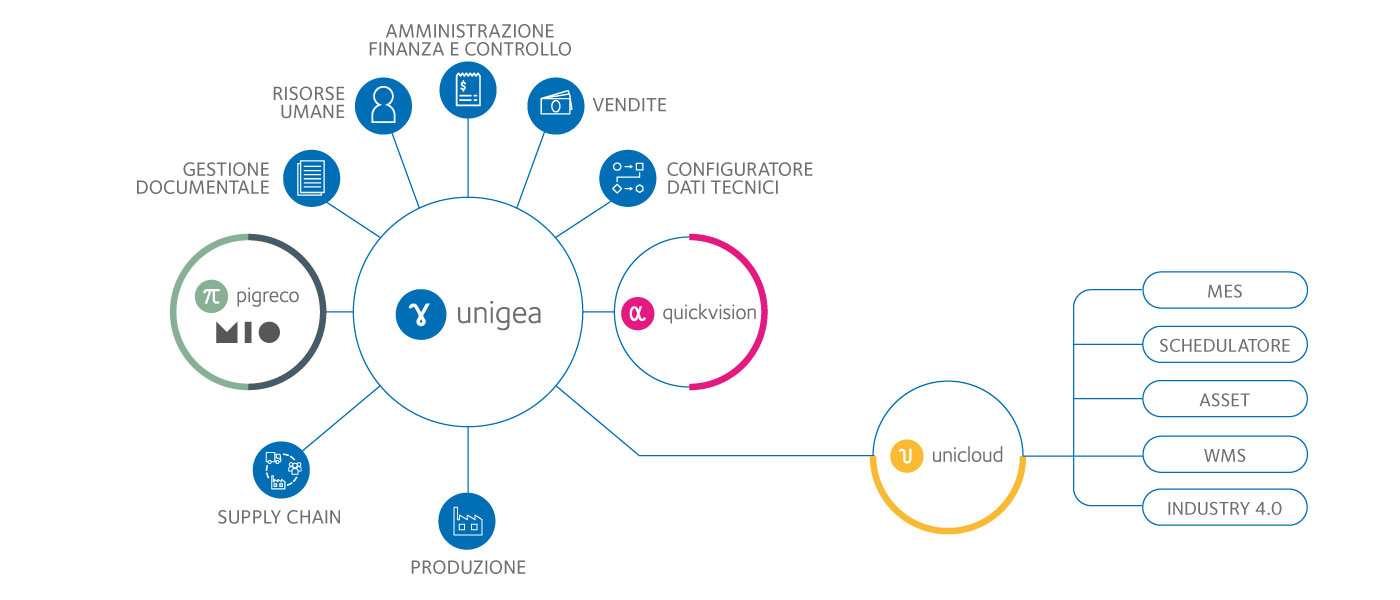
\includegraphics[width=1\textwidth]{soluzioni.jpg}
    \caption{Soluzioni di Deltasystem}
\end{figure}

\clearpage
%% Sottosezione
\subsection{UniCloud}

\begin{wrapfigure}{r}{0.38\textwidth}
    \begin{center}
        
\includegraphics[height=0.06\textheight]{unicloud.png}
    \end{center}
    \caption{Unicloud}
\end{wrapfigure}

%
\includegraphics[scale=0.15]{unicloud.png}

UniCloud è il framework proprietario di deltasystem. Creato per la digital transformation, viene utilizzato per lo svilupo di applicazioni aziendali basate sul cloud. 
La piattaforma facilita l’integrazione e l’estensione delle applicazioni aziendali sul web e su dispositivi mobili, permettendo una gestione dei processi scalabile, la centralizzazione dei dati e un elevata mobilità del software.


%\begin{wrapfigure}{l}{0.38\textwidth}
%    \begin{center}
%        
\includegraphics[width=0.38\textwidth]{unigea.png}
%    \end{center}
%    \caption{Unigea}
%\end{wrapfigure}



%% Sottosezione
\subsection{UniGea}

\begin{wrapfigure}{r}{0.38\textwidth}
    \begin{center}
        
\includegraphics[height=0.06\textheight]{unigea.png}
    \end{center}
    \caption{Unigea}
\end{wrapfigure}




       %% 
\includegraphics[scale=0.15]{unigea.png}


%\noindent
Basato su UniCloud, Unigea è un Erp esteso, cioè in grado di coprire tutte le aree aziendali, e unico, in grado di gestire diverse aree di business da un unica applicazione. Tale modularità permette una configurazione personalizzata in base alle esigenze del cliente.
Unigea, essendo completamente web based, fornisce un ambiente di facile apprendimento ed è accessibile da qualunque piattaforma, indipendentemente dall’hardware (anyclient-anywhere).
L’ERP Unigea è perfettamente integrato con tutte le altre soluzioni offerte da deltasystem.


%% Sottosezione
\subsection{Quickvision}
\begin{wrapfigure}{r}{0.38\textwidth}
    \begin{center}
        
\includegraphics[height=0.06\textheight]{quickvision.png}
    \end{center}
    \caption{Quickvision}
\end{wrapfigure}


%
\includegraphics[scale=0.15]{quickvision.png}

QuickVision è l’applicazione di data analytics per l'analisi interattiva, sintetica e flessibile delle informazioni aziendali, che trasforma in dati visualizzabili graficamente e comodamente navigabili.
Quickvision offre al cliente una piattaforma per consultare dati rapidamente tramite dashboard su misura con livello di dettaglio e filtri configurabili, consentendo quindi a ciascun utente di accedere solo alle informazioni a lui pertinenti.


%% Sottosezione
\subsection{Pigreco}

\begin{wrapfigure}{r}{0.38\textwidth}
    \begin{center}
        
\includegraphics[height=0.06\textheight]{pigreco.png}
    \end{center}
    \caption{Pigreco}
\end{wrapfigure}

%
\includegraphics[scale=0.4]{pigreco.png}

Configuratore tecnico-commerciale ideato per il mondo del mobile e dell'arredamento.
Permette la gestione grafica dell’intero ciclo di vita dell’ordine, dall’acquisizione alla produzione, sia prodotti standard che fuori misura, personalizzati o speciali.
Tale sistema è in grado di recepire le regole aziendali della composizione dei prodotti garantendo il rispetto dei parametri.
Pigreco è inoltre in grado di ottimizzare i flussi e i processi produttivi tramite la generazione di stampe tecniche, schemi di montaggio e liste di lavoro.
Infine Pigreco è dotato di un motore di rendering e un visualizzatore di modelli chiamato MyView.
MyView permette di visualizzare i modelli generati da Pigreco in ambientazioni realistiche e personalizzabili. Questa feature è compatibile con visori 3D per esplorare e analizzare il modello nel dettaglio.

%% Sottosezione
\subsection{MIO}
\begin{wrapfigure}{r}{0.38\textwidth}
    \begin{center}
        
\includegraphics[height=0.06\textheight]{mio.png}
    \end{center}
    \caption{MIO}
\end{wrapfigure}


%
\includegraphics[scale=0.2]{mio.png}

MIO è una piattaforma dedicata alle aziende del settore dell’arredamento nato dall’acquisizione di METAVERSO srl. 
È il primo virtual designer completo per l’arredo-casa.
Pensato per migliorare l’esperienza del cliente, tramite l’utilizzo di tecnologie 3D e realtà aumentata, MIO permette di creare e personalizzare prodotti ed ambienti con modelli ad alta fedeltà.
MIO si integra nativamente con ERP ed e-commerce. Genera ordini con distinta, codici prodotti e rendering, gestisce varianti di prodotto, prezzi e sconti rendendo le informazioni disponibili ai clienti in tempo reale.
Essendo anche MIO web-based ,è accessibile da qualunque browser senza necessità di plugin aggiuntivi. 
Fornisce anche informazioni sulle interazioni e scelte degli utenti per analizzare azioni e strategie di vendita.

%----------------------------------------------------
%% Fine dei capitoli normali, inizio dei capitoli-appendice (opzionali)
\appendix

%\part{Appendici}

\chapter{Titolo della prima appendice}
Sed purus libero, vestibulum ut nibh vitae, mollis ultricies augue. Pellentesque velit libero, tempor sed pulvinar non, fermentum eu leo. Duis posuere eleifend nulla eget sagittis. Nam laoreet accumsan rutrum. Interdum et malesuada fames ac ante ipsum primis in faucibus. Curabitur eget libero quis leo porttitor vehicula eget nec odio. Proin euismod interdum ligula non ultricies. Maecenas sit amet accumsan sapien.

%% Parte conclusiva del documento; tipicamente per riassunto, bibliografia e/o indice analitico.
\backmatter

%% Riassunto (opzionale)
%\summary
%Maecenas tempor elit sed arcu commodo, dapibus sagittis leo egestas. Praesent at ultrices urna. Integer et nibh in augue mollis facilisis sit amet eget magna. Fusce at porttitor sapien. Phasellus imperdiet, felis et molestie vulputate, mauris sapien tincidunt justo, in lacinia velit nisi nec ipsum. Duis elementum pharetra lorem, ut pellentesque nulla congue et. Sed eu venenatis tellus, pharetra cursus felis. Sed et luctus nunc. Aenean commodo, neque a aliquam bibendum, mauris augue fringilla justo, et scelerisque odio mi sit amet diam. Nulla at placerat nibh, nec rutrum urna. Donec ut egestas magna. Aliquam erat volutpat. Phasellus vestibulum justo sed purus mattis, vitae lacinia magna viverra. Nulla rutrum diam dui, vel semper mi mattis ac. Vestibulum ante ipsum primis in faucibus orci luctus et ultrices posuere cubilia Curae; Donec id vestibulum lectus, eget tristique est.

%% Bibliografia (praticamente obbligatoria)
\bibliographystyle{plain_\languagename}%% Carica l'omonimo file .bst, dove \languagename � la lingua attiva.
%% Nel caso in cui si usi un file .bib (consigliato)
\bibliography{thud}
%% Nel caso di bibliografia manuale, usare l'environment thebibliography.

%% Per l'indice analitico, usare il pacchetto makeidx (o analogo).

\end{document}

--- Istruzioni per l'aggiunta di nuove lingue ---
Per ogni nuova lingua utilizzata aggiungere nel preambolo il seguente spezzone:
    \addto\captionsitalian{%
        \def\abstractname{Sommario}%
        \def\acknowledgementsname{Ringraziamenti}%
        \def\authorcontactsname{Contatti dell'autore}%
        \def\candidatename{Candidato}%
        \def\chairname{Direttore}%
        \def\conclusionsname{Conclusioni}%
        \def\cosupervisorname{Co-relatore}%
        \def\cosupervisorsname{Co-relatori}%
        \def\cyclename{Ciclo}%
        \def\datename{Anno accademico}%
        \def\indexname{Indice analitico}%
        \def\institutecontactsname{Contatti dell'Istituto}%
        \def\introductionname{Introduzione}%
        \def\prefacename{Prefazione}%
        \def\reviewername{Controrelatore}%
        \def\reviewersname{Controrelatori}%
        %% Anno accademico
        \def\shortdatename{A.A.}%
        \def\summaryname{Riassunto}%
        \def\supervisorname{Relatore}%
        \def\supervisorsname{Relatori}%
        \def\thesisname{Tesi di \expandafter\ifcase\csname thud@target\endcsname Laurea\or Laurea Magistrale\or Dottorato\fi}%
        \def\tutorname{Tutor aziendale%
        \def\tutorsname{Tutor aziendali}%
    }
sostituendo a "italian" (nella 1a riga) il nome della lingua e traducendo le varie voci.
